\chapter{TINJAUAN PUSTAKA}
\label{chap:tinjauanpustaka}

% Ubah bagian-bagian berikut dengan isi dari tinjauan pustaka

Demi mendukung penelitian ini, dibutuhkan beberapa teori penunjang sebagai bahan acuan dan refrensi. Dengan demikian penelitian ini menjadi lebih terarah.

\section{Dasar Teori}
\label{sec:dasarteori}

\subsection{\textit{Artificial Intelligence}}
\label{artificialintelligence}

\subsection{\textit{Machine Learning}}
\label{machinelearning}

\textit{Machine Learning} adalah studi tentang algoritma komputer yang memberikan sistem kemampuan untuk belajar secara otomatis dan dapat meningkatkan kemampuan dari pengalaman yang sudah didapatkan \citep{machinelearning1}. Hal ini umumnya dilihat sebagai sub-bidang kecerdasan buatan. Algoritma pembelajaran mesin memungkinkan sistem membuat keputusan secara mandiri tanpa dukungan eksternal. Keputusan semacam itu dibuat dengan menemukan pola dasar yang berharga dalam data yang kompleks. Berdasarkan pendekatan pembelajaran, jenis data \textit{input} dan \textit{output}, dan jenis masalah yang dipecahkan, ada beberapa kategori utama dari algoritma \textit{machine learning} \textit{supervised, unsupervised} dan \textit{reinforcement learning}. Ada beberapa pendekatan hibrida dan metode umum lainnya yang menawarkan ekstrapolasi alami dari bentuk masalah pembelajaran mesin. Berikut merupakan penjelasan dari beberapa kategori utama dari algoritma \textit{machine learning}:

\begin{enumerate}
	\item \textit{Supervised Learning} diterapkan ketika data dalam bentuk variabel input dan nilai target output. Algoritma akan mempelajari fungsi pemetaan dari \textit{input} ke \textit{output}. Ketersediaan sampel data berlabel dengan skala besar mempunyai nilai yang tinggi dikarenakan masih terdapat kelangkaan \textit{dataset}. Pendekatan ini secara luas dapat dibagi menjadi dua kategori utama yaitu \textit{classification} dan \textit{regression}. Gambar \ref{fig:supervised} menampilkan visualisasi dari \textit{classification} dan \textit{regression} pada \textit{Supervised Learning}
	
	\begin{figure}[ht]
		\centering
		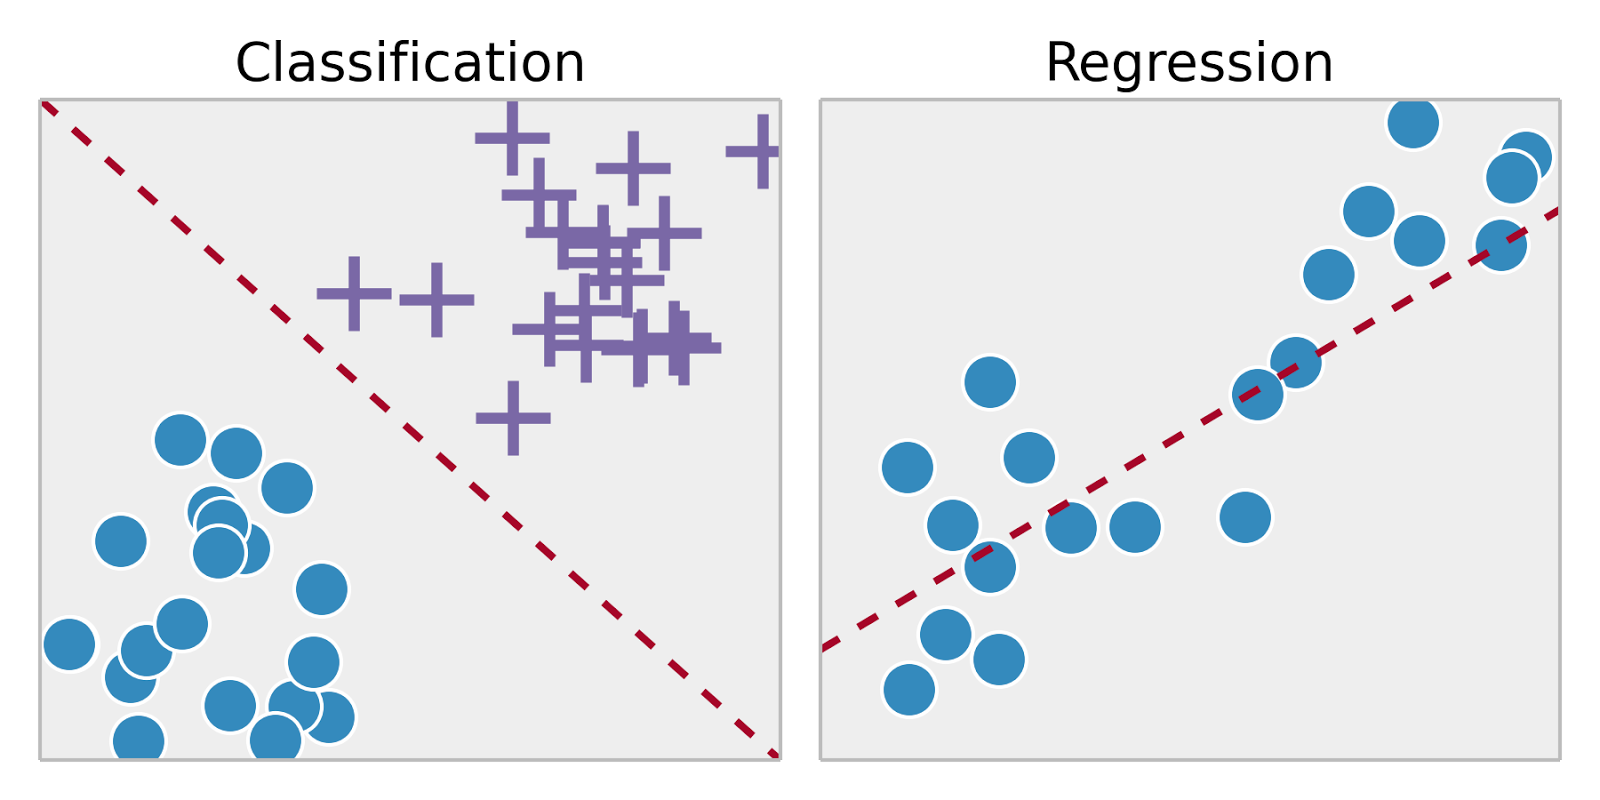
\includegraphics[scale=0.1]{gambar/supervised.png}
		\caption{Gambaran \textit{Supervised Learning}\citep{supervised}}
		\label{fig:supervised}
	\end{figure}  
	
	\item \textit{Unsupervised Learning} diterapkan ketika data hanya tersedia dalam bentuk \textit{input} dan tidak ada variabel \textit{output} yang sesuai. Algoritma semacam itu memodelkan pola yang mendasari data untuk mempelajari lebih lanjut tentang karakteristiknya. Salah satu jenis utama dari algoritma \textit{unsupervised} adalah pengelompokan. Dalam teknik ini, kelompok yang melekat dalam data ditemukan dan kemudian digunakan untuk memprediksi \textit{output} untuk \textit{input} yang tidak terlihat. Contoh dari teknik ini adalah untuk memprediksi perilaku pembelian pada pelanggan. Gambar \ref{fig:unsupervised} merupakan visualisasi dari algoritma \textit{unsupervised learning}.
	
	\begin{figure}[ht]
		\centering
		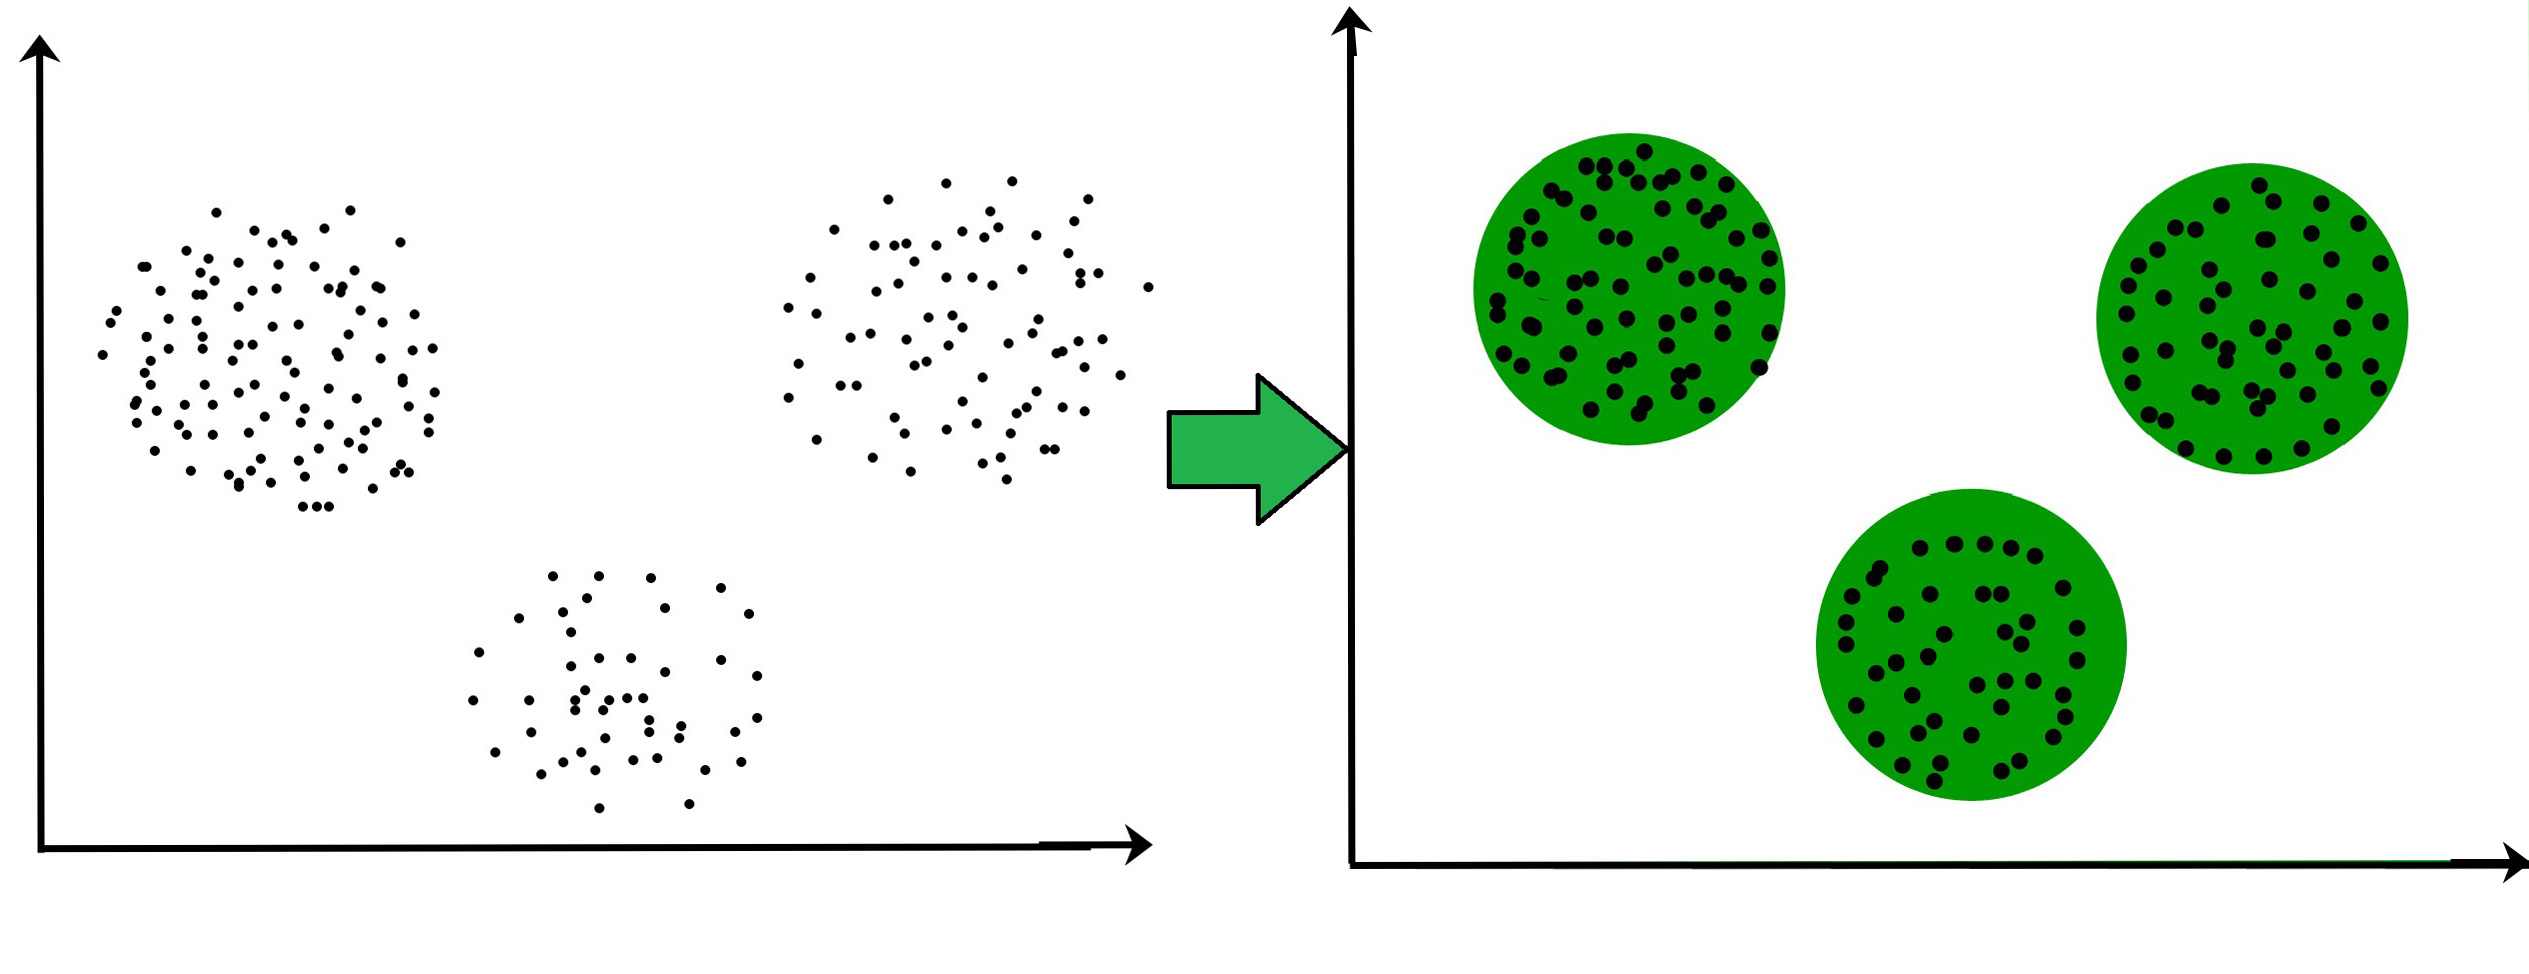
\includegraphics[scale=0.2]{gambar/unsupervised.jpg}
		\caption{Gambaran \textit{Unsupervised Learning}\citep{unsupervised}}
		\label{fig:unsupervised}
	\end{figure}
	
	
	\item \textit{Reinforcement learning} diterapkan ketika tugas yang ada
	adalah membuat urutan keputusan menuju \textit{reward} akhir. Selama proses \textit{learning}, \textit{artificial agent} mendapat \textit{reward} atau \textit{penalties} atas tindakan yang dilakukannya. Tujuannya adalah untuk memaksimalkan total \textit{reward} yang didapatkan. Gambar \ref{fig:reinforcement} merupakan visualisasi dari algoritma \textit{reinforcement learning}.
	
	\begin{figure}[ht]
		\centering
		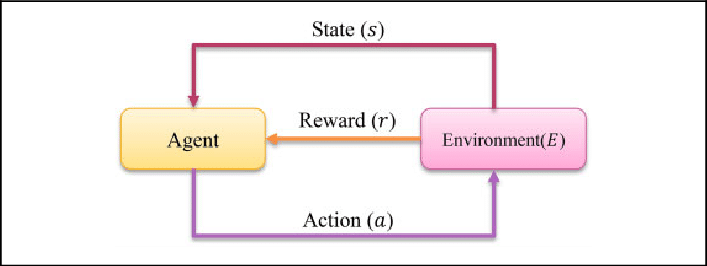
\includegraphics[scale=0.3]{gambar/reinforcement.png}
		\caption{Gambaran \textit{Reinforcement Learning}\citep{reinforcement}}
		\label{fig:reinforcement}
	\end{figure}
\end{enumerate}
